% !TeX spellcheck = de_DE
\section{Neuronale Netze}
\label{sec:neuroal_networks}
Klassische Algorithmen in der Informatik beschreiben, mit welchen Schritten ein spezielles Problem gelöst werden kann. In vielen Anwendungsfällen, wie zum Beispiel beim Sortieren einer Liste, verwenden Computersysteme diese und lösen das gegebene Problem schneller und effizienter als es Menschen möglich ist. Andere Aufgaben hingegen können von Menschen ohne Aufwand gelöst werden, stellen aber Computersysteme vor große Herausforderungen. Hierzu zählt unter anderem die Klassifizierung von Bildern. Ein Mensch kann beispielsweise Bilder von Hunden und Katzen unabhängig von Blickwinkel und Bildqualität unterscheiden beziehungsweise richtig zuordnen. Trotzdem ist es aufwendig, für solche Probleme klassische Algorithmen zu entwickeln, da die Lösung von vielen subtilen Faktoren abhängt \cite{kriesel2008kleiner}. Häufig werden in diesen Aufgabenfeldern \ac{KNN} eingesetzt, welche von biologischen neuronalen Netzen inspiriert sind und zum Forschungsgebiet des maschinellen Lernens gehören. Auch wenn die \ac{KNN} heute aktuell sind und viel Aufmerksamkeit erhalten, bildet die bereits 1943 veröffentlichte Arbeit von \citeauthor{mcculloch1943logical} die Grundlage für das Forschungsgebiet. In der Arbeit wird ein einfaches neuronales Netz mit Schwellwerten entwickelt, das die Berechnung von logischen und arithmetischen Funktionen ermöglicht \cite{mcculloch1943logical}. In den folgenden Jahrzehnten wurde die Funktionsweise der neuronalen Netze weiterentwickelt und der Einsatz in verschiedenen Aufgabenfeldern ermöglicht. Hierzu zählen neben der Klassifizierung von Bildern \cite{krizhevsky2012imagenet} unter anderem das Erkennen und die Interpretation von Sprache \cite{hinton2012deep}, \cite{andor2016globally} sowie das selbständige Lösen von Computer- und Gesellschaftsspielen \cite{mnih2013playing}, \cite{silver2016mastering}. Bevor im weiteren Verlauf dieses Kapitels auf den genauen Aufbau und die Funktionsweise von \ac{KNN} eingegangen wird, sind im Folgenden die biologischen neuronalen Netze vorgestellt.
\subsection{Biologische neuronale Netze}
\label{subsec:biological_neuraL_networks}
Das Forschungsgebiet der \ac{KNN} ist von den erfolgreichen biologischen neuronalen Netzen inspiriert, wie zum Beispiel dem menschlichen Gehirn \cite{kriesel2008kleiner}. In diesem Abschnitt werden die Eigenschaften betrachtet, die das Vorbild erfolgreich machen und für die \ac{KNN} übernommen werden sollen. Im Zuge dessen wird ein grober Überblick über die Struktur und Funktionsweise des menschlichen Gehirns gegeben. 
\\\\
Jede Sekunde erfassen die Rezeptoren des menschlichen Körpers unzählige Reize, wie zum Beispiel Licht, Druck, Temperatur und Töne. Die Reize werden anschließend elektrisch oder chemisch kodiert und über Nervenbahnen an das Gehirn geleitet, welches die Aufgabe hat, diese zu filtern, zu verarbeiten und entsprechend zu reagieren. Als Reaktion können zum Beispiel Signale an entsprechende Muskeln oder Drüsen gesendet werden \cite{kinnebrock2018neuronale}. Hierbei zeichnet sich das biologische neuronale Netz durch drei Eigenschaften aus, die klassische Algorithmen entweder nicht besitzen oder nur schwer umsetzen können. Ziel ist es, diese auf die \ac{KNN} zu übertragen \cite{kriesel2008kleiner}.
\begin{enumerate}
	\item \textbf{ Fähigkeit zu Lernen} \\
	Das menschliche Gehirn ist nicht wie ein klassischer Algorithmus für seine Aufgaben programmiert. Stattdessen besitzt es die Fähigkeit, durch Nachahmen oder Ausprobieren zu lernen \cite{kriesel2008kleiner}. Dafür wird das angestrebte Ergebnis mit dem tatsächlich erzielten verglichen und das Verhalten entsprechend angepasst. Dies ermöglicht es Menschen, verschiedene Aufgabengebiete erfolgreich zu lösen und sich ändernden Anforderungen anzupassen.
	
	\item \textbf{Fähigkeit zur Generalisierung}\\
	Auch für unbekannte Situationen findet das Gehirn meist plausible Lösungen, da es die Fähigkeit zur Generalisierung besitzt \cite{kriesel2008kleiner}. Das bedeutet, dass viele Situationen bereits bekannten Problemen zugeordnet werden können, mithilfe derer eine passende Verhaltensstrategie ausgewählt wird. 
	
	\item \textbf{Toleranz gegenüber Fehlern}\\
	Zudem zeichnen sich biologische neuronale Netze durch eine hohe Fehlertoleranz gegenüber verrauschten Daten aus. Beim zuvor genanntem Beispiel der Klassifizierung kann ein Teil des Bildes fehlen oder unscharf sein, trotzdem kann das abgebildete Motiv richtig zugeordnet werden.
\end{enumerate}

\subsubsection{Struktur des menschlichen Gehirns}
Das Forschungsgebiet der Neurowissenschaften befasst sich unter anderem mit dem menschlichen Gehirn, dessen Funktionsweise auch heute noch nicht vollständig erforscht ist. Dennoch ist schon seit 1861 durch die Arbeit von Paul Broca bekannt, dass es im menschlichen Gehirn verschiedene Regionen mit unterschiedlichen Aufgaben gibt \cite{russell2013kunstliche}. Zum Beispiel wird das sogenannte Kleinhirn (Cerebellum) für einen Großteil der motorischen Koordination verwendet, während das Großhirn (Telencephalon) unter anderem visuelle Reize empfängt \cite{kriesel2008kleiner}. Trotz der unterschiedlichen Aufgaben haben alle Bereiche des Gehirns einen gemeinsamen Grundbaustein, die sogenannten Neuronen \cite{russell2013kunstliche}. Im Folgenden wird der Aufbau und die Funktionsweise von diesen oberflächlich in Bezug auf die später vorgestellten künstlichen Neuronen betrachtet. Für einen vollständigen Überblick und eine genaue Beschreibung der Vorgänge ist auf entsprechende Fachliteratur zu verweisen.
\begin{figure}[h]
	\centering
	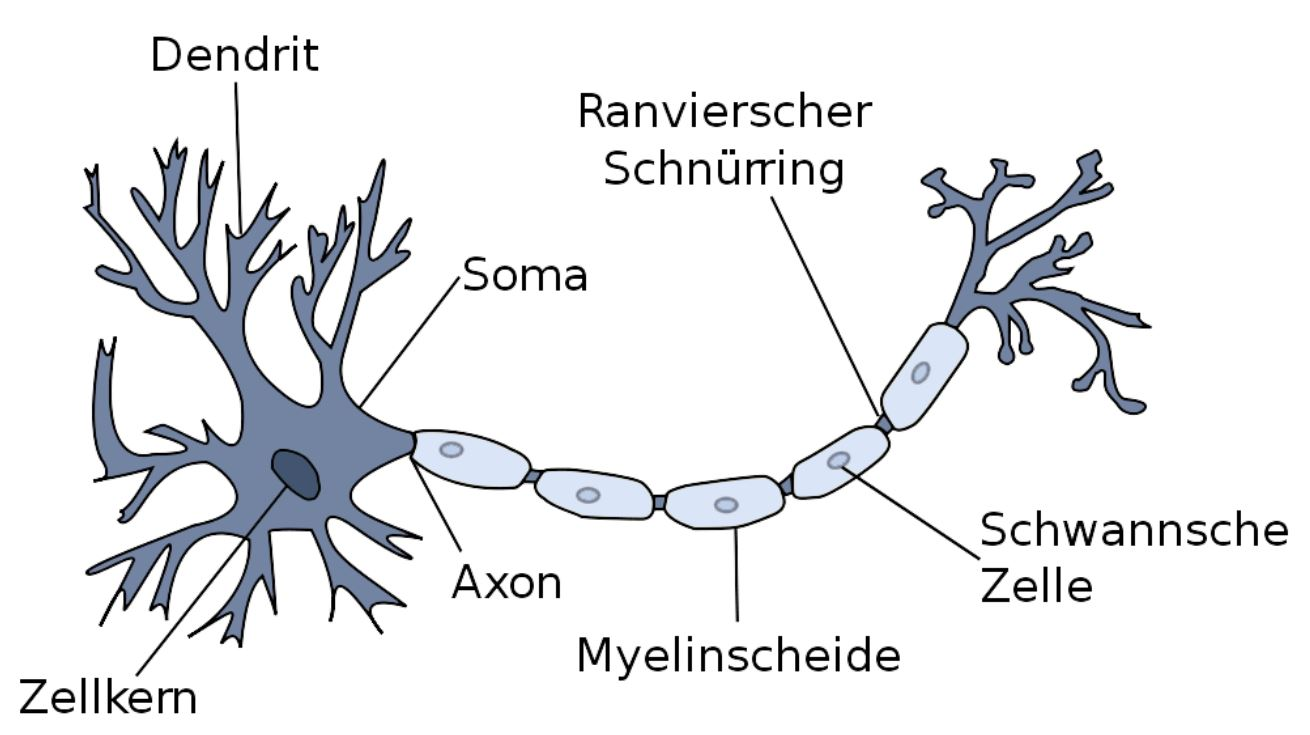
\includegraphics[width=0.75\textwidth]{./img/biologial_neuron.JPG} 
	\caption{Schematische Abbildung einer Nervenzelle \cite{kriesel2008kleiner}.}
	\label{fig:biological_neuron}
\end{figure}
\\ \noindent
Das menschliche Gehirn besitzt ungefähr ${10}^{11}$ einzelne Neuronen, deren schematischer Aufbau in Abbildung \ref{fig:biological_neuron} dargestellt ist. Jedes Neuron besitzt einen Zellkern, der sich im Zellkörper (Soma) befindet. Von dem Zellkörper gehen mehrere Fasern aus, die Dendriten genannt werden \cite{russell2013kunstliche}. An diesen befinden sich Synapsen, welche als Übertragungsstelle fungieren und elektrische oder chemische Signale von Rezeptoren oder anderen Neuronen empfangen \cite{kriesel2008kleiner}. Typischerweise empfängt ein Neuron Signale von 2000 bis 10.000 anderen Nervenzellen \cite{zell2003simulation}.  % TODO 3 mal empfangen
Synapsen, die elektrische Signale erhalten, haben eine starke, direkte, nicht regulierbare Verbindung vom Sender zum Empfänger. Diese sind für hart kodierte Verhaltensmechanismen nützlich, wie zum Beispiel den Fluchtreflex. Die chemische Synapse hingegen ist nicht direkt mit dem Sender verbunden, sondern durch den synaptischen Spalt getrennt. Zur Übertragung eines elektrischen Signals wird dieses auf der präsynaptischen Seite in ein chemisches Signal kodiert, indem Neurotransmitter freigesetzt werden. Diese können über den synaptischen Spalt übertragen und anschließend auf der postsynaptischen Seite wieder in ein elektrisches Signal kodiert werden. Ein großer Vorteil dieser Übertragungsart ist die Regulierbarkeit \cite{kriesel2008kleiner}. Verschiedene Neurotransmitter können unterschiedliche Effekte auf das Neuron haben, beispielsweise anregend (exzitatorisch) oder hemmend (inhibitorisch) wirken \cite{kirschbaum2008biopsychologie}. Zusätzlich kann die Menge der freigesetzten Neurotransmitter die Stärke des Signals beeinflussen \cite{kriesel2008kleiner}. Langfristig gesehen können auch neue Verbindungen bzw. Synapsen entstehen oder alte aufgelöst werden. Es wird angenommen, dass dies die Grundlage des Lernens im menschlichen Gehirn ist \cite{russell2013kunstliche}.
\\\\
Sowohl die anregenden als auch hemmenden Signale werden über die Dendriten an den Axonhügel weitergeleitet, welcher sich zwischen dem Soma und dem Axon befindet. Dort werden die Signale akkumuliert. Beim Überschreiten eines gewissen Schwellwerts wird ein elektrischer Impuls erzeugt, den das Axon weiterleitet \cite{kirschbaum2008biopsychologie}. Das Axon ist typischerweise einen Zentimeter, in Ausnahmen sogar bis zu einem Meter lang und wird von der Myelinscheide umgeben, die unter anderem Schutz vor mechanischer Überbeanspruchung bietet \cite{russell2013kunstliche}. Zusammen mit den Ranvierschen Schnürringen ermöglicht sie zudem eine schnellere Weiterleitung des Aktionspotenzials \cite{kirschbaum2008biopsychologie}. Das Axon endet mit dem sogenannten Endknopf, auch Axonterminal genannt. Dieses ist mit den Synapsen von anderen Neuronen verbunden und setzt beim Eintreffen eines Signals die Neurotransmitter frei, wodurch das Signal übertragen wird \cite{kirschbaum2008biopsychologie}. Typischerweise gibt ein einzelnes Neuron sein Signal an 1000 bis 10.000 andere Neuronen weiter, in Extremfällen sogar an bis zu 150.000 andere Neuronen \cite{zell2003simulation}, die alle parallel arbeiten. So entsteht ein großes und leistungsfähiges neuronales Netz. 

\subsection{Künstliche neuronale Netze}
\ac{KNN} sind ein mathematisches Modell, das im Vergleich zum biologischen Vorbild stark vereinfacht und idealisiert ist. Trotzdem können unterschiedliche mathematische Funktionen abgebildet werden. In diesem Kapitel werden die grundsätzliche Funktionsweise sowie die einzelnen Komponenten der \ac{KNN} vorgestellt.
\begin{figure}[h]
	\centering
	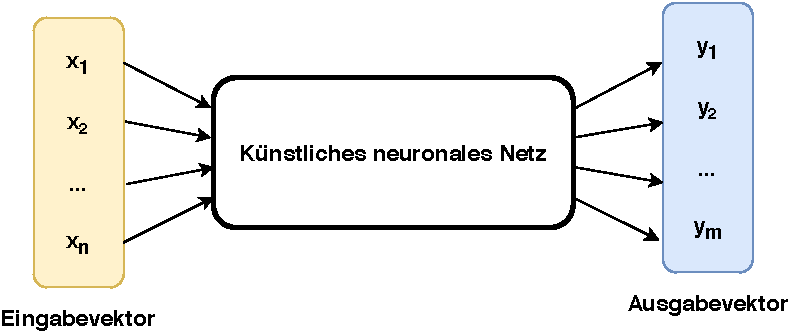
\includegraphics[width=0.6\textwidth]{./img/neural_network_basics/NeuralNetworkBlackbox.pdf} 
	\caption{KNN als Blackbox mit einem Eingabe- und Ausgabevektor}
	\label{fig:neural_network_blackbox}
\end{figure}
\\ \noindent
Betrachtet man ein \ac{KNN} als Blackbox (Abbildung \ref{fig:neural_network_blackbox}), gibt es eine gewisse Anzahl an Eingabewerten, die in einem Eingabevektor kodiert sind und eine Anzahl an Ausgaben, die in einem Ausgabevektor kodiert sind \cite{scherer2013neuronale}. Die Eingaben werden im Fall der \ac{KNN} nicht durch Rezeptoren erfasst, sondern sind durch ein Optimierungsproblem gegeben. Der Ausgabevektor soll das gewünschte Ergebnis enthalten. Je nach Optimierungsproblem kann die Interpretation von diesem variieren. Betrachtet man die Struktur der \ac{KNN}, sind einige Ähnlichkeiten zum biologischen Vorbild erkennbar. Diese werden im Folgenden genauer betrachtet \cite{zell2003simulation}:
\begin{enumerate}
	\item \textbf{Neuronen}\\
	Ähnlich zu den biologischen neuronalen Netzen, besteht auch das \ac{KNN} aus vielen Neuronen \cite{zell2003simulation}. Dies sind einfache Recheneinheiten, die primitive Funktionen bestimmen können \cite{scherer2013neuronale} und deren genaue Funktionsweise in Kapitel \ref{subsec:neuron} erläutert wird. Vorweggenommen sei, dass ein Neuron mehrere Eingabewerte besitzt, welche gewichtet sind und akkumuliert werden. Hierbei entsteht ein skalarer Ausgabewert, der den Aktivierungsgrad des Neurons repräsentiert und von anderen Neuronen als Eingabe verwendet werden kann \cite{kriesel2008kleiner}. 
	 
	\item \textbf{Gerichtete gewichtete Verbindungen}\\
	Wie in der Betrachtung der Neuronen angedeutet, sind diese über gerichtete Verbindungen miteinander vernetzt. Der Aktivierungszustand eines Neurons wird entsprechend der Verbindungen an die Zielneuronen weitergegeben, welche diesen Wert als Eingabe verarbeiten. Wie bei den biologischen neuronalen Netzen auch, können Eingaben unterschiedlich stark anregend oder hemmend wirken. Dies wird bei den \ac{KNN} über Gewichte in den Verbindungen realisiert \cite{zell2003simulation}.
	
	\item \textbf{Struktur und Gewichte}\\
	Der Ausgabevektor eines \ac{KNN} ist abhängig von der Struktur des Netzes und der Gewichte in den einzelnen Verbindungen.
	Für das erfolgreiche Lösen eines Optimierungsproblems muss ein \ac{KNN} die richtige Kombination aus Neuronen, Netzstruktur und gewichteten Verbindungen besitzen. Diese müssen durch Lernverfahren bestimmt werden, auf die in Kapitel \ref{subsec:optimization_strategies} näher eingegangen wird.
\end{enumerate}
Trotz der vorgestellten Ähnlichkeiten sind einige Unterschiede zwischen den biologischen neuronalen Netzen und den \ac{KNN} zu verdeutlichen, für die als Beispiel der Größenunterschied zu nennen ist. Das menschliche Gehirn mit seinen ${10}^{11}$ Neuronen besitzt pro Neuron ungefähr $10^4$ Verbindungen, wogegen die meisten \ac{KNN} nur ${10}^{2}$ bis ${10}^{4}$ Neuronen mit insgesamt ${10}^{5}$ Verbindungen besitzen. Auch werden keine chemischen Effekte, die auf benachbarte Neuronen wirken, sowie zeitliche und räumliche Lokalitätsprinzipien beachtet \cite{zell2003simulation}. Aus diesen Gründen sind die \ac{KNN} keine Nachbildung der biologischen neuronalen Netze, sondern verwenden diese ausschließlich als Inspiration. 

\subsection{Das Neuron}
\label{subsec:neuron}
In diesem Kapitel wird die Funktionsweise der einzelnen Neuronen betrachtet. Hierfür werden drei Phasen, die Propagierungsfunktion, die Aktivierungsfunktion sowie die Ausgabefunktion vorgestellt, in denen der Ausgabewert eines einzelnen Neurons berechnet wird. Betrachtet man ein \ac{KNN}, führen typischerweise mehrere Verbindungen zu einem Neuron $j$, welche von den Neuronen $i_1, i_2, ..., i_n$ ausgehen \cite{kriesel2008kleiner}. Dies ist schematisch in Abbildung \ref{fig:neuron_overview} dargestellt.
\begin{figure}[h]
	\centering
	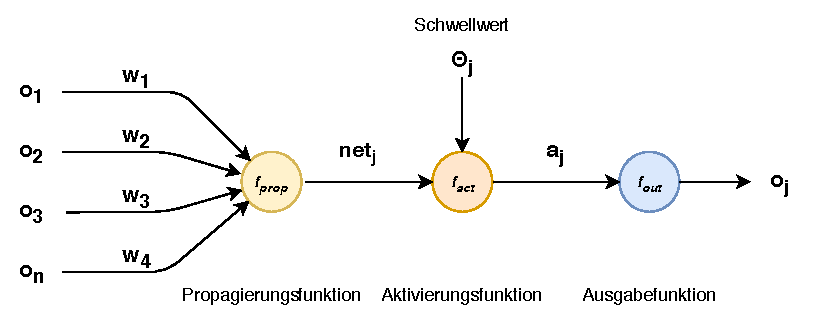
\includegraphics[width=0.9\textwidth]{./img/neural_network_basics/neuron_overview.pdf} 
	\caption{Schematische Darstellung eines einzelnen künstlichen Neurons}
	\label{fig:neuron_overview}
\end{figure}

\subsubsection{Propagierungsfunktion} 
Die Ausgabewerte $o_{i_1}, o_{i_2}, ..., o_{i_n}$ der Neuronen $i_1, i_2, ..., i_n$ werden als Eingabewerte für das Neuron $j$ verwendet. Für jeden Eingabewert existiert ein entsprechendes Gewicht $w_1, w_2, ..., w_n$ \cite{kriesel2008kleiner}. Somit repräsentiert $w_{ij}$ das Gewicht für die Verbindung von Neuron $i$ zu Neuron $j$ \cite{zell2003simulation}. Die Propagierungsfunktion $f_{prop}$ berechnet die Netzeingabe $net_j$, welche in der darauffolgenden Phase weiterverwendet wird \cite{kriesel2008kleiner}. 
$$net_j=f_{prop}(o_1, o_2, ..., o_n, w_1, w_2, ..., w_n)$$
Die meist verwendete Propagierungsfunktion, welche auch in den späteren Beispielen genutzt wird, ist die gewichtete Summe. Hierbei werden entsprechend der Formel die Werte $o_i$ mit dem entsprechenden Gewicht $w_i$ multipliziert und aufsummiert \cite{kriesel2008kleiner}:
$$net_j=\sum_{i}(o_{i} \cdot w_{i, j})$$

\subsubsection{Aktivierungsfunktion}
\label{subsubsec:activatoin_function}
Der Aktivierungszustand $a_j(t)$ gibt den Grad der Aktivierung von Neuron $j$ zum Zeitpunkt $t$ an. Ein neuer Aktivierungszustand zum Zeitpunkt $t+1$ wird mit der Aktivierungsfunktion $f_{act}$ berechnet. Diese berücksichtigt nicht nur die Netzeingabe $net_j(t)$, sondern auch den vorherigen Aktivierungszustand $a_j(t)$ und den Schwellwert $\Theta$ der Aktivierungsfunktion \cite{zell2003simulation}. Ein Schwellwert $\Theta_j$, auch \emph{Bias} genannt, ist dem Neuron $j$ zugeordnet und gibt die Stelle an, an welcher die Aktivierungsfunktion die größte Steigung hat \cite{kriesel2008kleiner}. Somit kann die Berechnung der Aktivierung $a_j(t+1)$ durch folgende Formel ausgedrückt werden \cite{zell2003simulation}:
$$a_j(t+1)=f_{act}(a_j(t), net_j, \Theta_j)$$
Bei der Berechnung kommt dem Schwellwert $\Theta$ eine besondere Bedeutung zu. Oftmals verwenden einige oder alle Neuronen eines \ac{KNN} dieselbe Aktivierungsfunktion, die Schwellwerte hingegen unterscheiden sich je nach Neuron. Des Weiteren sei angemerkt, dass die vorherige Aktivierung $a_j(t)$ je nach Netzstruktur oft keine Berücksichtigung bei der Berechnung findet \cite{kriesel2008kleiner}. Zudem wird in der Praxis bei Verwendung der gewichteten Summe als Propagierungsfunktion der Schwellwert eines Neurons oft schon in der ersten Phase miteinbezogen. Hierdurch ändert sich die Berechnung der Netzeingabe zu $net_j=\sum_{i}(o_{i} \cdot w_{i, j}) - \Theta_j$. Bei der Berechnung der Aktivierungsfunktion gilt dann $\Theta_j = 0$.
\\\\
Je nach Anwendungsgebiet können verschiedene Aktivierungsfunktionen mit unterschiedlichen Eigenschaften eingesetzt werden. Vier Beispiele sind im Folgenden vorgestellt, für die angenommen wird, dass $\Theta_j=0$ ist. Das einfachste Beispiel für eine Aktivierungsfunktion ist die sogenannte binäre Schwellwertfunktion, welche nur die Werte $0$ und $1$ zurückgeben kann \cite{kriesel2008kleiner}. Die Formel hierfür ist: 
$$
f_{act}(net_j)=\left\{\begin{array}{ll}
1 & \text { wenn } net_j \geq 0 \\
0 & \text { wenn } net_j < 0
\end{array}\right.
$$
Allerdings ist für diese Funktion der Wert der Ableitung immer $0$, ausgenommen an dem Schwellwert, an welchem sie nicht differenzierbar ist. Diese Eigenschaften machen sie ungeeignet für bestimmte Lernverfahren, wie zum Beispiel den Backpropagation Algorithmus, auf den in Kapitel \ref{subsec:backprop_algo} kurz eingegangen wird \cite{kriesel2008kleiner}. \\\\
Dieses Problem kann durch die Verwendung einer Sigmoidfunktion gelöst werden. Zwei bekannte Beispiele für Sigmoidfunktionen sind die logistische Funktion und der \ac{tanh} \cite{lecun2012efficient}. Die logistische Funktion kann Werte von 0 bis 1 annehmen und wird berechnet durch \cite{kriesel2008kleiner}: 
$$f_{act}(net_j)=\frac{1}{1+e^{-net_j}}$$
Allerdings können neuronale Netze je nach Verfahren schneller optimiert werden, wenn das durchschnittliche Gewicht aller Verbindungen nahe 0 ist. In diesem Fall kann die \ac{tanh}-Funktion besser geeignet sein, da sie Werte zwischen -1 und 1 annehmen kann \cite{lecun2012efficient}. Das abschließend vorgestellte Beispiel ist die sogenannte \emph{Rectifier}-Funktion. Diese wird oft in Zusammenhang mit dem Backpropagation Algorithmus erfolgreich eingesetzt \cite{glorot2011deep}. Berechnet wird sie durch:
$$f_{act}(net_j)= max(0, net_j)$$

\subsubsection{Ausgabefunktion}
Die Ausgabefunktion $f_{out}$ berechnet die Ausgabe $o_j$ von Neuron $j$. Als Eingabewert wird die Aktivierung $a_j$ verwendet \cite{zell2003simulation}. Definiert ist die Funktion durch:
$$o_j = f_{out}(a_j)$$
Ähnlich der Aktivierungsfunktion ist die Ausgabefunktion in der Praxis meist global für alle Neuronen definiert. Als eine solche Ausgabefunktion wird häufig die Identitätsfunktion verwendet, für welche $o_j = a_j$ gilt \cite{kriesel2008kleiner}. Diese kommt auch in den später vorgestellten Beispielen zur Anwendung. Ist die Ausgabe $o_j$ berechnet, kann sie als Eingabewert für andere verbundene Neuronen dienen.

\subsection{Netzstrukturen}
\label{subsec:network_structures}
Aus dem vorherigen Kapitel wird deutlich, dass die Gewichte einen großen Einfluss auf den Ausgabewert eines einzelnen Neurons haben. Der Ausgabevektor eines \ac{KNN} wird zusätzlich von der Anzahl an Neuronen sowie deren Verbindungsstruktur beeinflusst. Dieses Kapitel führt verschiedene Varianten ein, die je nach Optimierungsproblem eingesetzt werden können. 
\\\\
Typischerweise besitzt jedes \ac{KNN} Eingabe- und Ausgabeneuronen. Optional kann ein \ac{KNN} beliebig viele verdeckte Neuronen enthalten. Diese werden auch als \emph{Input}-, \emph{Output}- und \emph{Hidden}-Neuronen bezeichnet \cite{zell2003simulation}. Die Anzahl der Eingabe- und Ausgabeneuronen ist abhängig von der Größe des Eingabe- bzw. Ausgabevektors. Für jedes Element in den Vektoren gibt es ein entsprechendes Neuron.
Bei vielen Netzstrukturen werden die Neuronen des \ac{KNN} verschiedenen Schichten zugeordnet. In der ersten Schicht befinden sich die Eingabeneuronen, in der letzten die Ausgabeneuronen. Dazwischen befinden sich $n$ Schichten mit verdecken Neuronen \cite{zell2003simulation}. 
\\\\
Bei der Berechnung eines \ac{KNN} werden zuerst die Werte des Eingabevektors in die entsprechenden \emph{Input}-Neuronen eingesetzt. Anschließend werden alle Neuronen in einer bestimmten Reihenfolge aktiviert bzw. berechnet. Zuletzt bilden die Werte der \emph{Output}-Neuronen den Ausgabevektor. Die \emph{Hidden}-Neuronen, deren Bezeichnung darin begründet ist, dass ihr Ausgabewert nur ein Zwischenergebnis darstellt und vor dem Anwender verborgen bleibt, befinden sich zwischen den \emph{Input}- und \emph{Output}-Neuronen. Trotzdem sind sie ein elementarer Bestandteil der \ac{KNN} und bestimmen maßgeblich deren Leistungsfähigkeit. Beispielsweise kann ein aus \emph{Input}- und \emph{Output}-Neuronen bestehendes \ac{KNN} nur eine lineare Funktion repräsentieren. Ein \ac{KNN} mit einer ausreichend großen verdeckten Schicht kann jede beliebige kontinuierliche Funktion darstellen. Mit zwei Schichten kann ein \ac{KNN} sogar jede unstetige mathematische Funktion mit beliebiger Genauigkeit abbilden \cite{russell2013kunstliche}. Je nach Art des Verbindungsmusters zwischen den Neuronen werden \ac{KNN} einer von zwei Gruppen zugeordnet. Die erste Gruppe enthält Netze ohne Rückkopplung, welche auch \emph{feedforward}-Netze genannt werden. Die zweite Gruppe sind die sogenannten \emph{recurrent}-Netze, zu welchen \ac{KNN} mit Rückkopplungen gehören \cite{zell2003simulation}.

\subsubsection{Netze ohne Rückkopplung}
Die Definition der \emph{feedforward}-Netze sieht vor, dass es keine Verbindung geben darf, die von einem Neuron $j$ ausgeht und wieder zu diesem selbst führt. Dabei ist es irrelevant, ob eine direkte oder indirekte Verbindung über Zwischenneuronen besteht. Es entsteht ein azyklischer Graph \cite{zell2003simulation} und das \ac{KNN} kann infolgedessen keinen internen Zustand besitzen. Für die gleiche Eingabe wird immer dasselbe Ergebnis berechnet. Innerhalb dieser Kategorie gibt es zwei Untergruppen, die ebenenweise verbundenen \ac{KNN} und die \ac{KNN}, welche über sogenannte \emph{shortcut} Verbindungen verfügen.
\begin{figure}[h]
	\centering
	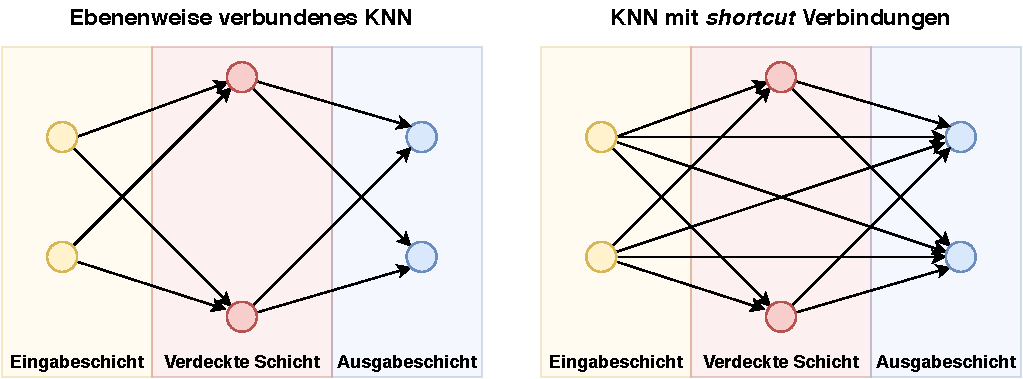
\includegraphics[width=1.0\textwidth]{./img/neural_network_basics/feed_forward_networks.pdf} 
	\caption{Links ein ebenenweise verbundenes \emph{feedforward} KNN, rechts ein KNN mit \emph{shortcut} Verbindungen}
	\label{fig:feed_forward_network_structures}
\end{figure}
Bei den rein ebenenweise verbundenen \ac{KNN} stammen die Eingabewerte eines Neurons immer aus der vorherigen Schicht. Der berechnete Ausgabewert eines Neurons wird nur an die Neuronen der nächsten Schicht weitergeleitet \cite{zell2003simulation}. Ein Beispiel hierfür ist in Abbildung \ref{fig:feed_forward_network_structures} links dargestellt. Im Gegensatz dazu stehen die \ac{KNN} mit \emph{shortcut} Verbindungen. Wie in Abbildung \ref{fig:feed_forward_network_structures} rechts dargestellt, können \emph{shortcut} Verbindungen eine oder mehrere Schichten überspringen. Für gewisse Optimierungsprobleme, unter anderem für das in Kapitel \ref{sec:analysis_valdation_functionality} dargestellte XOR-Problem, können so kleinere \ac{KNN} erzeugt werden \cite{zell2003simulation}. 

\subsubsection{Netze mit Rückkopplung}
Durch rückgekoppelte Verbindungen entstehen Zyklen in der Berechnung, wodurch sich das \ac{KNN} selbst beeinflussen kann. Damit ist unter anderem das Zwischenspeichern von Ergebnissen möglich \cite{russell2013kunstliche}. Somit kann die Berechnung des Ausgabevektors sowohl durch die Eingabewerte als auch durch die vorherigen Ergebnisse beeinflusst werden \cite{lin1998embedded}. Wie die \emph{feedforward}-Netze können auch die Netze mit Rückkopplungen je nach Verbindungsart verschiedenen Untergruppen zugeordnet werden \cite{zell2003simulation}. Diese sind in Abbildung \ref{fig:recurrent_network_structures} dargestellt und im Folgenden beschrieben.
\begin{figure}[h]
	\centering
	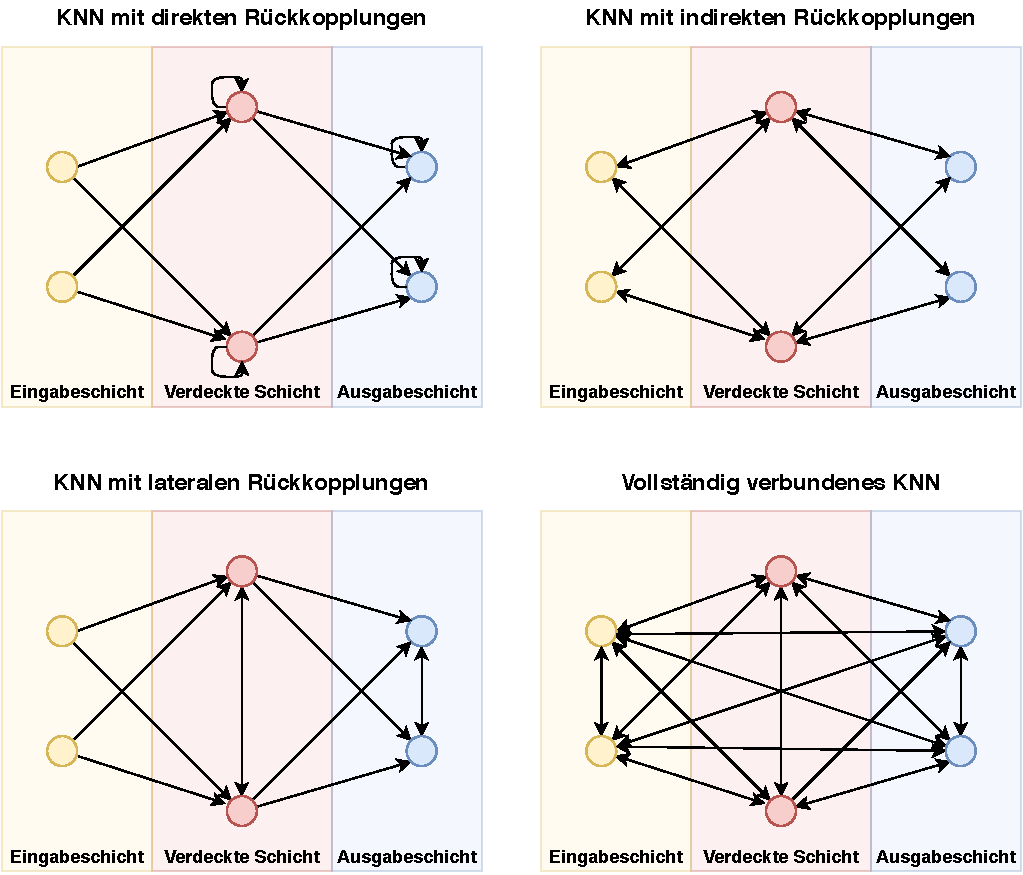
\includegraphics[width=1.0\textwidth]{./img/neural_network_basics/recurrent_networks.pdf} 
	\caption{Schematische Darstellung des Verbindungsmusters von verschiedenen KNN mit Rückkopplungen}
	\label{fig:recurrent_network_structures}
\end{figure}
\begin{enumerate}
	\item Bei \ac{KNN} mit direkten Rückkopplungen können Neuronen Verbindungen zu sich selbst haben und hierdurch ihre eigene Aktivierung verstärken oder abschwächen \cite{zell2003simulation}.
	\item Netze mit einer indirekten Rückkopplung erlauben im Gegensatz zu den \emph{feedforward}-Netzen auch Verbindungen in die vorherige Schicht \cite{zell2003simulation}. Wie bei der direkten Rückkopplung kann sich ein Neuron $j$ selbst beeinflussen, wenn es seinen Ausgabewert an ein Neuron $i$ der nächsten Schicht weiterleitet, welches eine Rückkopplung zu $j$ hat \cite{kriesel2008kleiner}.
	\item \ac{KNN} mit lateralen Rückkopplungen erlauben Verbindungen von Neuronen innerhalb einer Schicht, welche hemmend oder aktivierend wirken können. Oft entsteht dabei ein \emph{Winner-Takes-All}-Schema, da das beste Neuron alle anderen hemmt und sich selbst aktiviert \cite{kriesel2008kleiner}.
	\item Bei den vollständig verbundenen Netzen darf ein Neuron zu jedem anderen eine Verbindung besitzen. Ein Sonderfall sind hier die sogenannten Hopfield-Netze. Bei diesen müssen die Neuronen zu jedem anderen eine Verbindung besitzen mit Ausnahme zu sich selbst \cite{kriesel2008kleiner}.  
\end{enumerate}

\subsection{Optimierungsmöglichkeiten}
\label{subsec:optimization_strategies}
In den vorherigen Kapiteln ist aufgezeigt, dass das erfolgreiche Lösen eines Optimierungsproblems mit einem \ac{KNN} von vielen Faktoren abhängt. In der Praxis ist eine manuelle Bestimmung dieser bei komplexen Aufgaben nicht möglich. Aus diesem Grund muss ein Optimierungsverfahren, welches auch als Lernverfahren bezeichnet wird, angewendet werden. Ziel hierbei ist, einen Teil oder alle Parameter des \ac{KNN} durch einen Algorithmus automatisch zu bestimmen. Typischerweise ist das Lernverfahren unabhängig vom eigentlichen Optimierungsproblem und kann daher in verschiedenen Bereichen ohne großen zusätzlichen Aufwand eingesetzt werden. 
\\\\
Ein Lernverfahren kann theoretisch auf vier verschiedene Arten die Eigenschaften eines \ac{KNN} optimieren \cite{zell2003simulation}. Diese sind im Folgenden kurz zusammengefasst.
\begin{enumerate}
	\item \textbf{Modifizieren der Verbindungsgewichte}:\\
	Die Gewichte der einzelnen Verbindungen werden in der Praxis von allen Lernverfahren optimiert \cite{zell2003simulation}. Gründe hierfür sind, dass ein \ac{KNN} mehrere Millionen Verbindungen besitzen kann, welche unmöglich manuell optimiert werden können, und dass die Gewichte entscheidend für die erfolgreiche Optimierung sind.

	\item\textbf{Modifizieren der Schwellwerte}:\\
	Die Schwellwerte der Neuronen werden wie die Gewichte von den meisten Lernverfahren optimiert. In der Praxis ist der hierbei verwendete Vorgang oft identisch mit der Gewichtsoptimierung. Dies ist möglich, wenn, wie in einigen Implementierungen umgesetzt, die Schwellwerte durch Gewichte repräsentiert werden. Hierzu wird einem \ac{KNN} ein sogenanntes \emph{Bias}-Neuron hinzugefügt, welches immer den Wert 1 hat. Von diesem gehen Verbindungen zu allen Neuronen aus. Der Schwellwert $\Theta_j$ von einem Neuron $j$ wird durch das Gewicht $w_{\Theta j}$ repräsentiert. Dieses ist der eingehenden Verbindung vom \emph{Bias}-Neuron zugeordnet, sodass gilt $1\cdot w_{\Theta j} = \Theta_j$. Dadurch muss bei der Berechnung eines Neurons der Schwellwert nicht mehr explizit miteinbezogen werden, sondern wird im Rahmen der Propagierungsfunktion indirekt mit den anderen gewichteten Eingaben verarbeitet. Bezüglich der Optimierung wird die Verbindung zum \emph{Bias}-Neuron wie andere gewichtete Verbindungen behandelt \cite{zell2003simulation}.

	\item \textbf{Hinzufügen und Entfernen von Verbindungen oder Neuronen}:\\
	Das Hinzufügen beziehungsweise Entfernen von Verbindungen und Neuronen ist im Vergleich zu den bereits vorgestellten Möglichkeiten aufwendig und in der Umsetzung schwieriger. Daher ist es in vielen bekannten Algorithmen nicht implementiert. Bei diesen muss die Struktur mithilfe von Expertenwissen oder Erfahrung festgelegt werden \cite{stanley2017oreilly}, andernfalls ist eine geeignete Struktur experimentell zu ermitteln. Da dieses Vorgehen häufig nicht effizient ist, gibt es dennoch einige Algorithmen, die das Hinzufügen und Entfernen von Strukturen bei der Optimierung nutzen. Diese gehören oft zu der Klasse der neuroevolutionären Algorithmen, auf welche in Kapitel \ref{subsec:neuroevolution} eingegangen wird \cite{kriesel2008kleiner}.
	
	\item \textbf{Ändern der Propagierungs-, Aktivierungs- und Ausgabefunktion}:\\
	Die Optimierung der verwendeten Propagierungs-, Aktivierungs- und Ausgabefunktion ist theoretisch möglich, die Umsetzung ist in der Praxis allerdings nicht sehr verbreitet \cite{zell2003simulation}. Auch in dieser Arbeit werden diese Funktionen nicht durch einen Algorithmus angepasst und daher nicht weiter betrachtet. 
\end{enumerate}

\subsection{Arten von Optimierungsverfahren}
\label{subsec:learning_in_neural_networks}
In Kapitel \ref{subsec:optimization_strategies} sind Optimierungsmöglichkeiten aufgelistet, welche von einem Lernverfahren in der sogenannten Trainingsphase des \ac{KNN} angepasst werden können. Ziel ist, dass am Ende dieser Phase der Ausgabevektor des \ac{KNN} dem gewünschten Ergebnis entspricht. Voraussetzung hierfür ist, dass das gewünschte Ergebnis erkennbar ist \cite{zell2003simulation}. Bei den Lernverfahren wird grundsätzlich zwischen dem überwachten, unüberwachten und bestärkenden Lernen differenziert, welche unterschiedliche Arten des Lernens für verschiedene Aufgabenstellungen repräsentieren. Im Folgenden wird ein Überblick über diese gegeben. Für eine genaue Beschreibung und die dazugehörigen Algorithmen wird auf entsprechende Fachliteratur verwiesen.

\subsubsection{Überwachtes Lernen}
\label{subsubsec:supervised_learning}
Das überwachte Lernen, auch \emph{supervised learning} genannt, wird häufig mit dem Backpropagation Algorithmus und seinen Derivaten umgesetzt und beruht auf bekannten Beispieldaten. Diese müssen in großer Anzahl schon vor dem Lernvorgang vorhanden sein und den Eingabevektor sowie den gewünschten Ausgabevektor des \ac{KNN} enthalten \cite{zell2003simulation}. In der sogenannten Trainingsphase analysiert das Lernverfahren die vorhanden Beispieldaten mit dem Ziel, Muster zu extrahieren. Am Ende der Trainingsphase soll das \ac{KNN} nicht nur die korrekte Lösung für die bekannten Beispiele angeben können, sondern auch für ähnliche, unbekannte Eingabedaten. Damit ist die Eigenschaft der Generalisierung erfüllt. \cite{zell2003simulation}. Um den Erfolg des Verfahrens zu überprüfen, werden die Beispieldaten in Trainings- und Testdaten unterteilt. Die Trainingsphase wird nur mit den Trainingsdaten durchgeführt, sodass die Testdaten dem \ac{KNN} unbekannt sind. Ist diese Phase abgeschlossen, weil beispielsweise das \ac{KNN} eine gute Genauigkeit erreicht hat, werden die Testdaten zur Validierung eingesetzt. Hierbei wird überprüft, ob das \ac{KNN} auch für unbekannte Eingabevektoren die richtigen Ergebnisse berechnet \cite{kriesel2008kleiner}. Diese Art des Lernens ist im Vergleich zu den anderen Varianten sehr schnell \cite{zell2003simulation}, aber das Anwenden ist nicht in jeder Situation möglich. Liegen keine Beispiele vor, kann das \ac{KNN} nicht trainiert werden. Sind die Beispieldaten fehlerhaft oder verrauscht, kann das Training langsam, nicht zufriedenstellend oder unmöglich sein.

\subsubsection{Unüberwachtes Lernen}
\label{subsubsec:unsupervised_learning}
Beim unüberwachten Lernen, auch \emph{unsupervised learning} genannt, stehen ebenfalls Beispieldaten zur Verfügung, allerdings enthalten diese nur den Eingabevektor und keine dazugehörigen Ausgabevektoren. Ziel solcher Lernverfahren ist, Muster in den Eingabedaten automatisch zu erkennen und diese verschiedenen Gruppen zuzuordnen, sodass ähnliche Eingabewerte derselben Gruppe zugewiesen werden \cite{zell2003simulation}. Solche Verfahren können einige Vorteile gegenüber dem überwachten Lernen bieten \cite{mahmad2005IEEE}. Zum Beispiel müssen vor dem Training keine Beispieldaten mit Ausgabevektoren vorliegen, welche teilweise sehr teuer und aufwendig zu erstellen sind. Des Weiteren kann je nach Algorithmus die Anzahl an vorhandenen Gruppen automatisch zugewiesen werden. So können auch unterschwellige Muster, die nicht von einem Menschen erkannt werden würden, die Zuweisung beeinflussen \cite{mahmad2005IEEE}.
 
\subsubsection{Bestärkendes Lernen}
\label{subsubsec:reinforcment_learning}
Die letzte Klasse ist das bestärkende Lernen, auch \emph{reinforcment learning} genannt. Typischerweise wird diese Art des Lernens in dynamischen Umgebungen eingesetzt, in welcher ein sogenannter Agent mit einer Umgebung interagiert. Ein häufig genannter Begriff in diesem Kontext ist der \ac{MDP}, welcher in Abbildung \ref{fig:mdp_problem} dargestellt ist und anhand dessen im Folgenden das bestärkende Lernen beschrieben ist \cite{sutton2018reinforcement}. 
\begin{figure}[h]
	\centering
	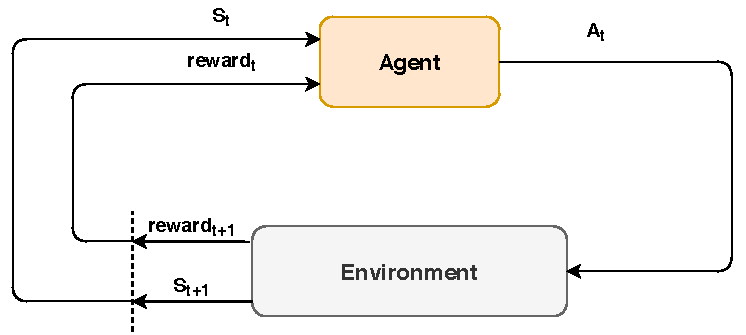
\includegraphics[width=0.7\textwidth]{./img/neural_network_basics/mdp.pdf} 
	\caption{Interaktion des Agenten mit der Umgebung im MDP}
	\label{fig:mdp_problem}
\end{figure}
\\ \noindent
Zwei wichtige Grundkomponenten des \acp{MDP} sind der Agent und die Umgebung. Der aktuelle Zustand der Umgebung zu einem Zeitpunkt $t$ wird durch die Variable $S_t$ repräsentiert. Ist die Umgebung zum Beispiel ein Computerspiel, kann $S_t$ unter anderem die aktuelle Position sowie Zielkoordinaten enthalten. Der Zustand $S_t$ steht dem Agenten zur Verfügung, der daraufhin eine Aktion $A_t$ ausführt. Als Basis für die Entscheidung kann ein \ac{KNN} dienen, welches als Eingabevektor den aktuellen Zustand verwendet und einen Ausgabevektor mit der gewählten Aktion erzeugt. Die verfügbaren Aktionen sind je nach System unterschiedlich. So können zum Beispiel bei der Steuerung von Robotern sowohl direkte Steuersignale für die Motoren ausgegeben werden als auch \emph{high-level} Entscheidungen wie die Bewegungsrichtung. Nach Ausführung der Aktion wird der Zustand der Umgebung entsprechend angepasst und ein neuer Zustand $S_{t+1}$ entsteht \cite{sutton2018reinforcement}, für den der Agent eine neue Aktion auswählen kann. Zusätzlich wird ein Belohnung, auch als $reward$ bezeichnet, vergeben. Dies ist ein numerischer Wert, der angibt, wie richtig oder falsch die gewählte Aktion war \cite{zell2003simulation}. Eine richtige Aktion zeichnet sich dadurch aus, dass sie den Agenten näher an sein gewünschtes Ziel bringt. Im zuvor genannten Beispiel des Computerspiels ist der \emph{reward} größer, wenn der Agent die Distanz zum Ziel verringert und kleiner bzw. negativ, wenn der Agent sich wieder entfernt. Ziel eines Optimierungsalgorithmus ist, die Summe der erhaltenen Belohnungen zu maximieren. Hierdurch ergeben sich komplexe Anforderungen an das Lernverfahren. Bei der Entscheidung, welche Aktion $A_t$ bei einem Zustand $S_t$ den meisten Erfolg verspricht, muss sowohl der direkte als auch zukünftige \emph{reward} berücksichtigt werden \cite{sutton2018reinforcement}. Dies ist notwendig, da ein Agent viele Aktionen in derselben sich ändernden Umgebung ausführt und eine Entscheidung Auswirkungen auf die Zukunft hat. Somit kann es bei vielen Optimierungsproblemen  lohnenswert sein, zur Schaffung einer besseren Ausgangslage zuerst eine schlechte Belohnung in Kauf zu nehmen, wenn dadurch im weiteren Verlauf größere Belohnungen erreicht werden können. Eine weitere Herausforderung für solche Algorithmen ist, dass ein Gleichgewicht zwischen dem Nutzen von Erfahrung und Ausprobieren gefunden werden muss. Möglichst hohe Belohnungen kann ein Agent nur erhalten, wenn er bekannte Entscheidungen trifft, die in der Vergangenheit erfolgreich waren. Allerdings müssen auch neue unbekannte Aktionen ausgewählt werden, da diese unter Umständen besser sein können. Für ein gutes Lernverfahren ist es notwendig, eine Kombination aus beidem zu ermöglichen \cite{sutton2018reinforcement}. Bei vielen Optimierungsproblemen wird das bestärkende Lernen erfolgreich eingesetzt. Ein Nachteil jedoch ist die lange Laufzeit im Vergleich zu anderen Verfahren, wie zum Beispiel dem überwachten Lernen. Grund hierfür ist, dass eine niedrige Belohnung keine Aussage darüber trifft, wie das \ac{KNN} optimiert werden muss, um bessere Ergebnisse zu erzielen. Anpassungen können sich sowohl positiv als auch negativ auf den Agenten auswirken \cite{zell2003simulation}. 

\subsection{Backpropagation Algorithmus}
\label{subsec:backprop_algo}
Das Backpropagation Verfahren ist ein bekanntes und weit verbreitetes Lernverfahren, welches häufig im Zusammenhang mit dem überwachten Lernen verwendet wird. Dieses Kapitel stellt das Verfahren oberflächlich vor. Es ist anzumerken, dass nur die generellen Konzepte genannt werden und auf eine genaue Beschreibung verzichtet wird. Der Grund hierfür ist, dass das Verfahren im weiteren Verlauf der Arbeit nicht verwendet wird. Für einen genauen Überblick ist auf entsprechende Fachliteratur verwiesen \cite{zell2003simulation}.
\\\\
Ziel des Backpropagation Verfahrens ist die Optimierung der Verbindungsgewichte und Schwellwerte. Die Struktur des \ac{KNN} wird nicht angepasst. Eine weiterer wichtiger Unterschied zu den später vorgestellten neuroevolutionären Algorithmen ist, dass bei der Trainingsphase nur ein \ac{KNN} benötigt wird. Im Zusammenhang mit dem überwachtem Lernen wird über die Beispieldaten iteriert. Für die Eingabedaten berechnet das \ac{KNN} die vermuteten Ausgabewerte. Danach wird der Fehler zwischen dem erhaltenen und erwarteten Ergebnis gebildet. In Abhängigkeit der Größe des Fehlers, werden die Gewichte und Schwellwerte direkt angepasst, sodass der Fehler insgesamt geringer wird. Dieser Vorgang wird solange wiederholt, bis das \ac{KNN} die gewünschte Genauigkeit bietet. Häufig ist dieses Verfahren beim finden einer Lösung sehr schnell. Jede Änderung ist gerechtfertigt und sollte die Leistung des \ac{KNN} verbessern bzw. den Fehler verringern.  

%Während der Optimierung erhält das \ac{KNN} Beispieldaten, für welche der Ausgabevektor berechnet wird. Für das berechnete %Ergebnis wird ein Feedback gegeben, welches auch als \emph{reward} bezeichnet wird. Dieses gibt an, ob der Ausgabewert korrekt %ist beziehungsweise wie richtig oder falsch. Das Lernverfahren muss mit diesen Angaben das \ac{KNN} optimieren, kann aber nicht %wissen wie die Gewichte und je nach Algorithmus die Struktur verändert werden müssen. Dies ist auch der Grund, warum diese Art %des Lernens im Vergleich zum überwachtem Lernen sehr langsam ist, da die Gewichte nicht gezielt angepasst werden können %\cite{zell2003simulation}.\\
%Das Einsatz

% Agent Scenario, Agent must explore/take known actions = trade off, Reward funktion ist anpassbar, muss nicht so sein. 
% file:///D:/Dropbox/Studium%20Master/Semester%203/Masterthesis%20Quellen/Neuroevolution%20strateies%20for%20episodic%20reinforcment%20learning.pdf
% "C:\Users\Simon Hauck\Downloads\Neuroevolution strateies for episodic reinforcment learning.pdf"